\section{High-dimensional stress-test protocols}
\label{app:highdimensional_confirmation}

\paragraph{Lorenz--96.}
The fixed-data chaotic forecasting comparison uses the standard Lorenz--96 system with
forcing $8$, $d_x=128$, and all coordinates observed. One generated
dataset (seed $20{,}260{,}719$) is fixed across ten model-initialization
seeds and contains $128/32/64$ train/validation/test trajectories with 201
stored states each. The stored interval is $0.05$, training observations
receive noise at $5\%$ of the training scale, and the declared forecast
horizons $1,5,10,25,50,100$ therefore extend through physical time $5$.
Both KAEs use a four-times overcomplete lift, $d_z=512$, 20-step training
windows, 3,000 updates, batch size 1,024, and a full trainable latent matrix.
Forecasts encode only the initial state and then repeatedly apply the learned
$K$ without periodic decode--encode refresh.
The deterministic references are persistence, ordinary DMD, and rank-32
truncated DMD fitted to the same fixed dataset.

The exact-dense control uses tanh in every hidden encoder and decoder layer and
a linear latent output. It contains no ReLU, GELU, soft-shrinkage, or dropout
module; its sparsity coefficient, weight decay, transition penalty, and
soft-block penalty are zero; and it uses Adam rather than AdamW. All ten
fail-closed audits pass. At an absolute activation threshold of $10^{-4}$,
its empirical latent density is $0.9996$, compared with $0.4884$ for the
signed LISTA KAE. Thus this comparison does not obtain a nominally dense row
through an activation that itself creates zeros. It remains a complete-recipe
comparison: sign splitting mechanically permits at most one active coefficient
per pair, LISTA and MLP encoders and decoder normalization differ, and the
signed/dense models have 459,264/443,136 parameters. Mean training times were
approximately 85.5/34.9 seconds under the common update budget.

At physical times $2.5$ and $5$, sparse mean NRMSE is $0.8987$ and
$0.9669$, versus $0.9595$ and $1.2889$ for exact dense. Paired mean
relative reductions are $6.30\%$ (95\% model-seed bootstrap interval
$[5.09\%,7.32\%]$) and $24.87\%$
($[22.98\%,26.51\%]$); sparse wins all ten paired seeds. Exact two-sided
sign-flip tests give $p=0.001953$ at each horizon and Holm adjustment over
the two declared long horizons gives $p=0.003906$. Sparse also has lower
mean NRMSE than persistence, DMD, and truncated DMD at both horizons. Since
the dataset is fixed, this inference quantifies model-initialization
variability conditional on one generated dataset, not variability over new
Lorenz--96 datasets.

\paragraph{Four-well vector Allen--Cahn representation packet.}
The synthetic physics-motivated multibasin study evolves two fields on a periodic
$16\times16$ grid under diffusion coefficient $0.005$ and a four-well
reaction potential. This gives $d_x=2(16)^2=512$; both KAEs use the required
four-times overcomplete $d_z=2{,}048$ lift. RK4 integration uses step
$0.005$, every twentieth state is stored, and the $512/128/256$
train/validation/test trajectories extend to 200 stored transitions, or
physical time $20$. Models train without basin labels or counts on fields
through physical time $12$; the longer fields measure whether forecasts and
supports remain meaningful well beyond a short observation interval. The
evaluation-only fate label is the modal final well at time $20$.

The comparison includes a direct tanh circular-convolutional forecaster, an
exact-dense convolutional KAE, and a signed sparse convolutional KAE. The
dense KAE has tanh hidden activations, a linear latent output, a full
$2{,}048\times2{,}048$ transition, Adam, and zero coefficients for ordinary
sparsity, temporal group sparsity, weight decay, transition stability, and
soft-block regularization. No zero-inducing activation or dropout is present;
all ten dense audits pass. Its holdout active density at threshold $10^{-4}$
is $0.998$, versus $0.499$ for the selected sign-split temporal-support model.

The first sealed test showed finite-time fate information but fragmented
within-fate families: sparse transfer coverage was $0.988$, ARI was $0.704$, and
normalized $H(F\mid B)/H(F)=0.396$ exceeded the frozen $0.35$ ceiling. Once
opened, that test became development evidence. A label-free temporal-group
objective had already been implemented and frozen before test access as the
sole architectural fallback; the failed result triggered its validation
screen rather than motivating a new post-test objective. For a
sampled 20-state training window, it penalizes the sum over latent coordinates
of each coordinate's root-mean-square activation across time. The screened
weights were $10^{-3},3\times10^{-3},10^{-2},3\times10^{-2}$; the weakest
weight was the only row selected because it passed all six frozen checks on
the original validation data. More broadly, validation fate metrics had
selected physical-time-20 scoring and family Jaccard $0.40$, and three screen
checks---ARI and the two normalized conditional entropies---selected the
temporal weight. The recipe is therefore label-assisted. No fate label, basin
count, or trajectory assignment enters the objective, encoding,
representative fitting, or family assignment conditional on these selected
hyperparameters.

The selected weight was then evaluated as one fixed roster of ten fresh
initialization seeds using the same label-assisted validation fate gates; no
seed was omitted, and the entire ten-seed packet had to pass. Mean
validation transfer coverage was $0.961$, normalized
$H(B\mid F)/H(B)=0.110$, normalized $H(F\mid B)/H(F)=0.299$, ARI was
$0.756$ (95\% model-seed bootstrap interval $[0.702,0.798]$), NMI was
$0.784$, and purity was $0.936$. Sparse beat exact dense in all ten paired
ARI comparisons ($p=0.001953$, exact two-sided sign flip), satisfying every
frozen promotion check. Only then was a new dataset generated with a different
simulation seed. Support representatives were formed without labels from
absolute-threshold masks on even-indexed trajectories of the original
validation set and transferred at fixed Jaccard $0.40$; they were never refit
on the new data. Thus map formation and new-simulation-seed holdout assignment remain
label-free after validation-selected recipe freezing; the new 256 test initial
conditions and their labels are used only for scoring.

On this new-initial-condition dataset, sign-split temporal-support transfer coverage is $0.982$.
Its all-256 ARI treats unassigned family $-1$ as a category rather than dropping
uncovered trajectories; this all-trajectory statistic is $0.767$ (95\% interval
$[0.742,0.787]$). NMI is $0.730$, purity
is $0.923$, and normalized $H(B\mid F)/H(B)=0.151$. Exact dense transfers one
threshold-support family and has ARI and NMI zero; this shows that the support
extractor finds no dense partition, not that dense latent values contain no
fate information. Sparse wins all ten paired support-ARI comparisons
($p=0.001953$). Across all 256 trajectory final states, the normalized
$H(F\mid B)/H(F)=0.359$ ($[0.339,0.382]$) misses its $0.350$ ceiling by
$0.009$ and the map has a mean 10.8 families. Both the support family and
modal-well fate label are computed from the $T=20$ final field: this is not
$x_0$ fate prediction or alignment throughout each trajectory. This
prespecified primary gate therefore fails and was not moved after test access.

After the earlier opened test exposed mixed-domain fragmentation but before
opening the new holdout, we prospectively froze a single-well-dominated
final-field slice: a trajectory is retained when at least
$90\%$ of its final grid occupies its modal Allen--Cahn well. The criterion
uses the new-simulation-seed holdout fate label only to stratify evaluation. It retains
130/256 trajectories and all four modal-well fates. On this slice, every one
of the ten sparse model seeds transfers exactly four families with ARI, NMI,
and purity $1.000$ and both normalized conditional entropies zero. This is
exactly one transferred support family per finite-time fate on the declared
slice, not proof of geometric basin-interior membership. Residual family
fragmentation is associated with spatially mixed, interface-rich final fields.

\begin{figure*}[tbp]
\centering
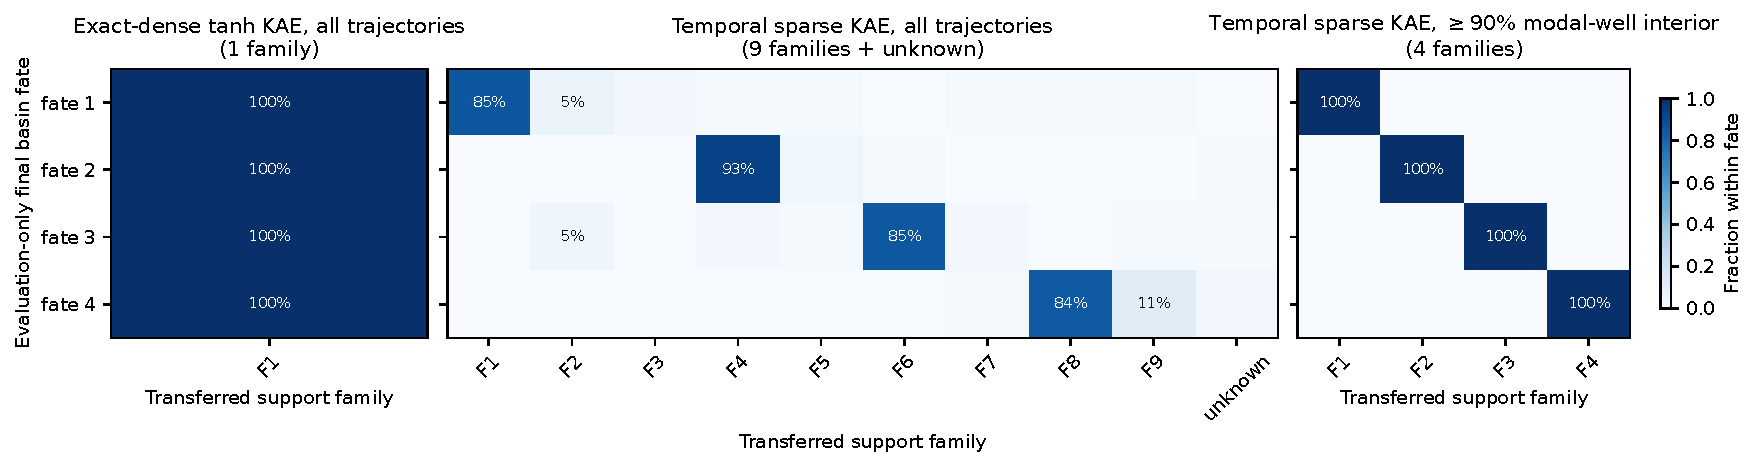
\includegraphics[width=\textwidth]{figures/neurips_paper_2026/fig_allen_cahn_support_contingency.pdf}
\caption{Row-normalized final-state fate--support contingency for the fixed
display seed on the new-simulation-seed Allen--Cahn holdout. Exact dense assigns every
fate to one family (left). Temporal sparse has one dominant family per fate on
all trajectories but additional families in mixed-domain fields (center). On
the single-well-dominated final-field slice prospectively frozen for this new
holdout after earlier mixed-domain fragmentation, it transfers exactly
four families in one-to-one correspondence with the four finite-time
modal-well fates (right). Aggregate claims use all ten
model seeds, not this display seed alone. Columns preserve the raw
training-codebook family IDs in numeric order, independent of evaluation fate;
row labels give panel-specific trajectory counts;
the center and right panels share one family axis, so blank right-panel columns
are families absent from the declared slice.}
\label{fig:allen_cahn_support_contingency}
\end{figure*}

Forecasts are evaluated at physical times $0.1,0.5,1,2,4,8,12,16,20$, so
the display does not rely on a nominally multi-step but physically negligible
horizon. Temporal sparse has lower error than dense through time $4$, but the
ordering reverses at time $8$ and remains reversed. At time $20$, direct,
dense, and sign-support final field MSE are $0.0293$, $0.1184$, and
$0.2991$; their final RMSE ratios to persistence are $0.218$, $0.442$, and
$0.649$. All three learned rows beat persistence, but the direct control is
best. This separates the high-dimensional sparse forecasting claim, which
comes from Lorenz--96 and the separate packet below, from this physics-based
multibasin representation claim. The temporal-support model's pre-split group
activity is nearly complete, so it is not evidence of intrinsic coefficient
sparsity before its sign split.

\paragraph{Separate forecast-optimized global-$K$ packet.}
This experiment shares the $d_x=512,d_z=2{,}048$, grid, stored interval, and
four-well system, but it is a different trained model and dataset split. It
uses 512 training trajectories, full 200-step sequences, batch size 8, 2,000
autoencoder-pretraining updates, and 3,500 forecast-training updates. Adam has
learning rate $3\times10^{-4}$ for the network and $10^{-6}$ for $K$, with
zero weight decay. The selected soft-thresholded recipe uses shrinkage $0.15$, ordinary
elementwise sparsity weight $0.01$, and zero temporal-group penalty. The dense
arm uses tanh hidden activations, a linear latent output, a full trainable $K$,
and zero sparsity, shrinkage, dropout, weight decay, transition, or block
penalties; all ten fail-closed audits pass. An exact checkpoint audit finds
the same trainable tensor shapes/count and shared convolutional, decoder, and
$K$ backbone, with $12{,}698{,}690$ trainable parameter entries in both arms.
The nominal $2{,}048^2$ LISTA recurrence matrix stays exactly zero and is inert
with one LISTA loop, leaving $8{,}504{,}386$ effective forward-path parameters
per arm. Thus the treatment is jointly soft-thresholding at $0.15$ and an
$L_1$ weight of $0.01$ under matched parameter count and backbone, not equal
function-class capacity or an isolated component test.

Selection used a three-seed, four-recipe development screen. The selected
recipe was then trained for seeds 64--73 and scored on 256 fresh initial
conditions from simulation seed $20{,}260{,}724$, using no basin label or
count. Checkpointing used the even development partition and joint H160/H200
endpoints; held-out scoring uses all fresh validation trajectories and no
checkpoint reselection. Forecasting is direct
repeated-$K$ rollout without re-encoding. Mean near-zero fraction at threshold
$10^{-3}$ is $0.434$ for sparse and $0.0025$ for dense. All 20 runs are finite;
mean active A100L utilization is $95.55\%$ (range $90.56$--$96.78\%$).
On the opened development screen, the one-pass soft-thresholded sparse arm had lower through-horizon mean
and terminal MSE than its same-recipe dense arm in all 16 comparisons across
the four forecast-weighting/latent-consistency recipes. This is descriptive
screen robustness, not confirmation or a threshold-versus-$L_1$ ablation.

\begin{table}[tbp]
\centering
\caption{Separate forecast-optimized Allen--Cahn comparison. ``Mean'' averages
field MSE over every forecast state through the horizon; it is not an
unnormalized cumulative sum. Intervals resample paired model seeds. The
one-sided max-$t$ values are a multiplicity sensitivity, not a replacement for
the failed internally frozen four-cell gate.}
\label{tab:allen_cahn_global_k_forecast_optimized}
\resizebox{\textwidth}{!}{\begin{tabular}{llrrrrl}
\toprule
Horizon & Endpoint & Dense & Sparse & Reduction & Wins & Marginal 95\% CI; max-$t$ $p$ \\
\midrule
H160 & Mean through H & 0.04503 & 0.04220 & 6.3\% & 8/10 & [2.6, 9.5]\%; 0.014 \\
H160 & Terminal & 0.05189 & 0.05065 & 2.4\% & 7/10 & [-1.6, 6.0]\%; 0.197 \\
H200 & Mean through H & 0.04731 & 0.04472 & 5.5\% & 8/10 & [1.7, 8.8]\%; 0.019 \\
H200 & Terminal & 0.06086 & 0.05890 & 3.2\% & 7/10 & [-0.8, 6.7]\%; 0.112 \\
\midrule
\multicolumn{7}{l}{\footnotesize Matched trainable tensor shapes and effective forward-path parameter count; sparse jointly applies soft-thresholding $0.15$ and $L_1$ weight $0.01$.} \\
\multicolumn{7}{l}{\footnotesize Internally frozen confirmation gate: failed; sealed holdout not generated or opened.} \\
\bottomrule
\end{tabular}
}
\end{table}

At H160, sparse/dense through-horizon mean field MSE is
$0.04220/0.04503$; at H200 it is $0.04472/0.04731$. These are reductions of
$6.30\%$ and $5.48\%$, each with 8/10 paired wins. Terminal reductions are
$2.38\%$ and $3.22\%$, each with 7/10 wins and an interval crossing zero.
The corresponding through-horizon MSE ratios to persistence are
$0.0958/0.1023$ at H160 and $0.0938/0.0993$ at H200 for sparse/dense;
terminal ratios are $0.0824/0.0844$ and $0.0937/0.0968$. Thus the physical
times 16--20 are nontrivial relative to persistence even though the terminal
sparse--dense effect remains uncertain.
The rule frozen before fresh confirmation-data generation required all four
mean and terminal cells to pass; it failed.
In addition to both terminal intervals crossing zero, H200 terminal misses the
minimum $5\%$ reduction and 8/10-win criteria.
The conditional seed-$20{,}260{,}725$ holdout was never generated or opened.

\paragraph{Same-checkpoint new-initial-condition robustness check.}
After the preceding four-cell decision failed, we prospectively froze the
already positive H200 through-horizon endpoint. This endpoint choice was
outcome-aware. We crossed the same ten sparse and ten dense checkpoints with
three newly generated datasets (simulation seeds $1{,}775{,}404{,}171$,
$74{,}732{,}421$, and $293{,}789{,}188$), each containing 256 trajectories.
There was no retraining, checkpoint reselection, periodic re-encoding, label
use, or basin-count use. The rollout encodes once and applies the unchanged
global $K$ for 200 steps, reaching physical time 20. Datasets are averaged
within each paired model seed before inference, so the inferential unit remains
the ten paired checkpoint seeds rather than the 30 crossed seed--dataset cells.

Sparse/dense through-horizon field MSE is $0.04616/0.04903$, a $5.86\%$
reduction with 8/10 paired-seed wins. A 100,000-resample paired-seed bootstrap
interval is $[2.40\%,9.21\%]$ and the exact one-sided paired sign-flip value is
$9/1{,}024=0.00879$. Dataset-specific reductions are $4.68\%$, $5.88\%$, and
$7.03\%$, all in the same direction; these three values are descriptive rather
than independent hypothesis tests. H200 terminal error is descriptive only:
$0.06476/0.06683$, a $3.09\%$ reduction with 7/10 wins. A separate authenticated
recomputation exactly reproduced all primary values and authenticated the
complete 60-cell roster, all 20 checkpoints, and all three datasets. The
result establishes same-checkpoint robustness to new initial conditions in
this fixed PDE condition. It does not retroactively repair the original
four-cell gate or establish terminal, parameter, resolution, physics, or
system generalization. Descriptively, across the full physical-time trace, the
sparse arm-mean instantaneous MSE is lower at all 200 times, but the
running-mean reduction declines from about 14\% early to 5.86\% at $T=20$.
Over the late half, $T=10.1$--20, sparse/dense instantaneous means are
$0.05216/0.05380$, only a $3.06\%$ reduction; no simultaneous curve-wide
inference is claimed. The result remains a
trajectory-average rather than terminal or asymptotic advantage. H200 equals
the trained temporal horizon and is not extrapolation beyond it.

\begin{figure*}[tbp]
\centering
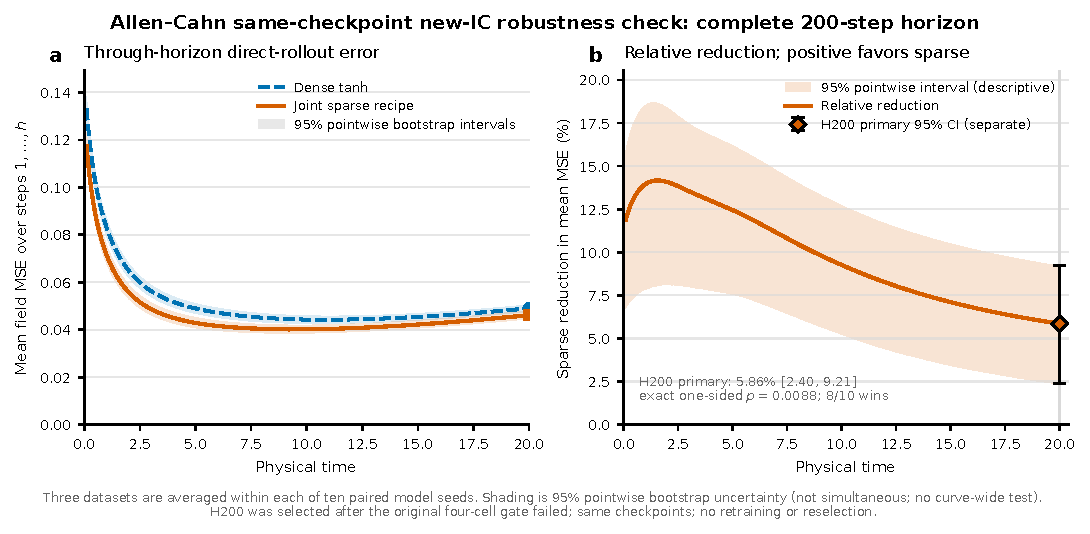
\includegraphics[width=\textwidth]{figures/neurips_paper_2026/fig_allen_cahn_new_ic_replication_full_horizon.pdf}
\caption{Complete 200-step Allen--Cahn same-checkpoint new-initial-condition
robustness trace. H200 was selected after the original four-cell gate failed;
the checkpoints were neither retrained nor reselected.
The left panel reports mean field MSE over steps $1,\ldots,h$ against physical
time. The right panel reports the ratio-of-arm-means reduction. Shading is a
descriptive pointwise 95\% paired-seed bootstrap band and is neither
simultaneous nor a curve-wide test; the black H200 interval is the separate
100,000-resample primary interval. Datasets are averaged within each of ten
paired model seeds.}
\label{fig:allen_cahn_new_ic_full_horizon}
\end{figure*}

\paragraph{Outcome-aware physical concordance on the same forecasts.}
On the identical 20 checkpoints, three datasets, 256 trajectories per dataset,
and 200-step direct rollouts, sparse is directionally better at the H200
cumulative endpoint on all seven frozen secondary metrics. Pixel nearest-well
disagreement, well-area total-variation error, interface-edge disagreement,
full-free-energy error, and gradient-energy error fall by
$4.61\%$, $6.07\%$, $2.25\%$, $6.20\%$, and $8.58\%$, respectively, and
survive Holm correction across all seven metrics. Modal-well accuracy rises by
$0.236$ percentage points and potential-energy error falls by $3.77\%$, but
their Holm-adjusted values are $0.303$ and $0.119$ and their intervals include
zero. Thus the result is broad phase-assignment, interface, and thermodynamic
concordance, not seven statistically significant endpoints.

Every metric was frozen and computed for every trajectory and time. Pixel and
modal-well scores use the four known wells only for evaluation; well-area error
compares the four phase fractions; interface error compares periodic nearest-
well boundary indicators; and the energy terms use the discrete Lyapunov
functional whose derivative matches the pinned reaction--diffusion generator.
Datasets are first averaged within model seed, leaving ten paired checkpoint
seeds as the inferential units. Exact one-sided paired sign flips are Holm-
adjusted as one seven-metric family, and intervals resample paired seeds. No
periodic re-encoding, fate label, basin count, finite-prefix filtering, or
trajectory exclusion alters a forecast.

\begin{table*}[t]
\centering
\small
\caption{Outcome-aware, same-checkpoint secondary Allen--Cahn analysis showing all seven frozen metrics at the H200 cumulative endpoint. Effects are relative reductions for the six lower-is-better errors and percentage-point differences for modal accuracy. Confidence intervals are paired-seed 95\% intervals for the oriented absolute effect; $q$ is Holm-adjusted across all seven metrics. Bold $q$ values are at most 0.05.}
\label{tab:allen_cahn_physics_metrics}
\begin{tabular}{lrrrrr}
\toprule
Metric & Dense & Sparse & Oriented effect & Wins & Holm $q$ / abs. 95\% CI \\
\midrule
Pixel phase error & 0.09424 & 0.08990 & 4.61\% & 9/10 & \textbf{0.0146} / [0.00229, 0.00610] \\
Modal-well accuracy & 0.90742 & 0.90977 & +0.236 pp & 5/10 & 0.3027 / [-0.00551, 0.01061] \\
Well-area TV error & 0.05402 & 0.05074 & 6.07\% & 8/10 & \textbf{0.0352} / [0.00112, 0.00535] \\
Interface-edge error & 0.09966 & 0.09742 & 2.25\% & 9/10 & \textbf{0.0146} / [0.00118, 0.00311] \\
Free-energy error & 0.02843 & 0.02667 & 6.20\% & 10/10 & \textbf{0.0068} / [0.00112, 0.00243] \\
Potential-energy error & 0.03597 & 0.03462 & 3.77\% & 8/10 & 0.1191 / [-0.00006, 0.00311] \\
Gradient-energy error & 0.02897 & 0.02649 & 8.58\% & 10/10 & \textbf{0.0068} / [0.00164, 0.00332] \\
\bottomrule
\end{tabular}
\end{table*}


\begin{figure*}[tbp]
\centering
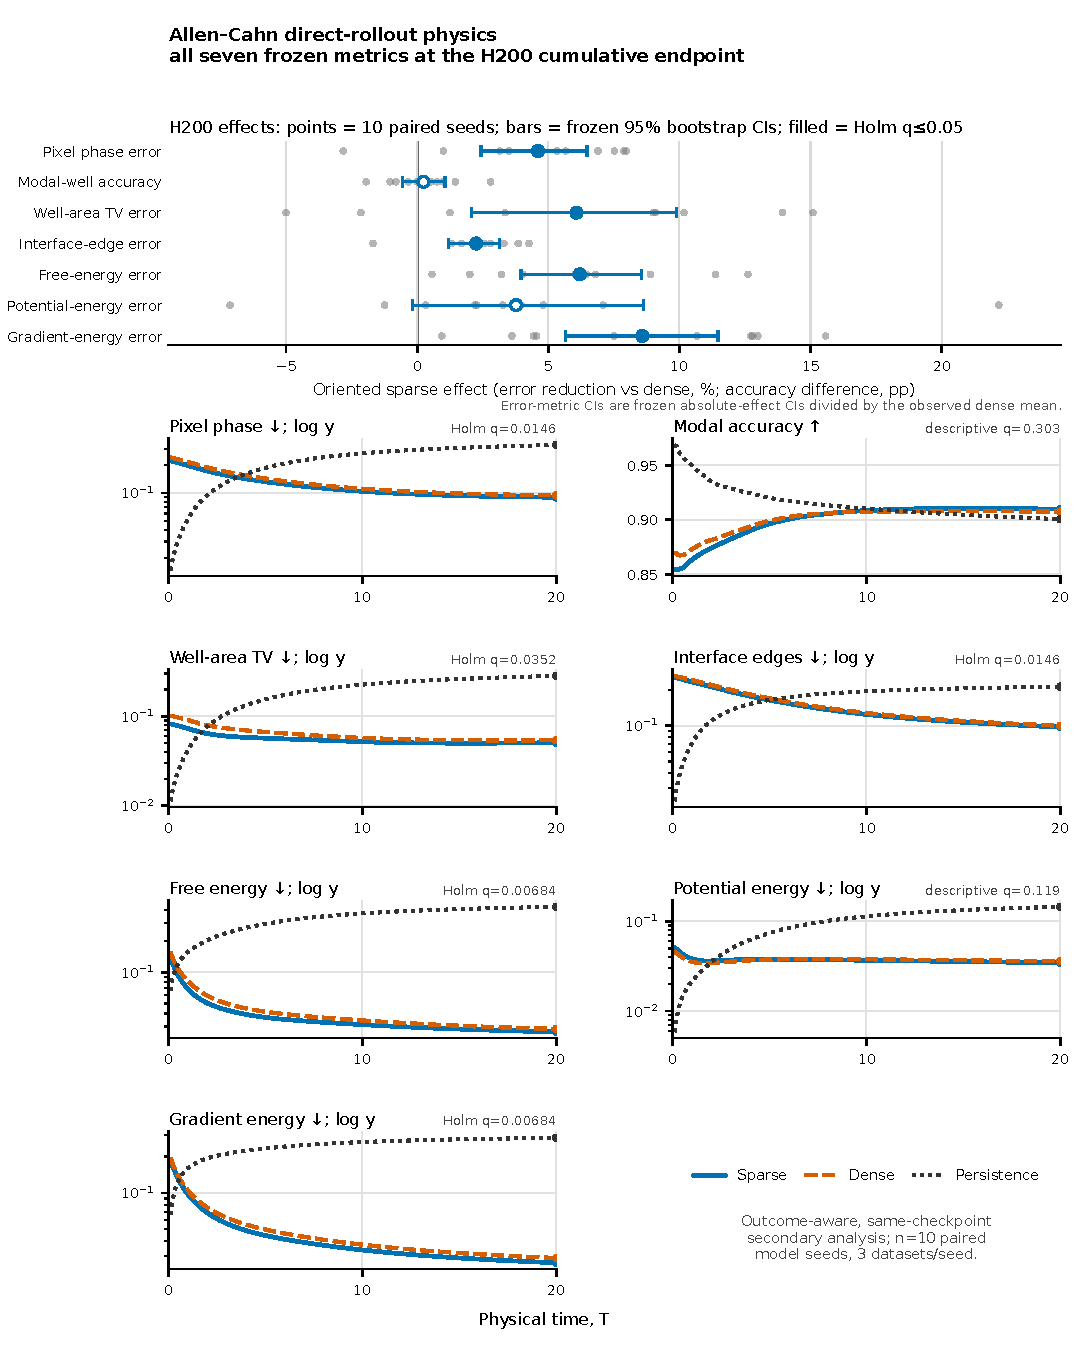
\includegraphics[width=0.94\textwidth]{figures/neurips_paper_2026/fig_allen_cahn_physics_metrics.pdf}
\caption{All seven frozen Allen--Cahn physical metrics on the same-checkpoint
new-initial-condition forecasts. The top panel shows the H200 cumulative
oriented effect, all paired-seed effects, and paired-seed intervals; filled
marks survive seven-way Holm correction. Lower panels show every arm-mean
curve through physical time 20, including persistence. Curves are descriptive;
the statistical family consists of the seven H200 cumulative endpoints. The
analysis is outcome-aware because H200 and these checkpoints were retained
after the original four-cell forecasting gate failed.}
\label{fig:allen_cahn_physics_metrics}
\end{figure*}

This translation addresses whether lower field MSE merely reflects benign
amplitude changes: the favorable interface and separated potential/gradient
energy components argue against that narrow explanation in this condition.
It does not identify a sparse component as causal, repair the original gate,
establish terminal superiority, or generalize over retraining, PDE parameters,
grid resolution, or another physical system. The appropriate next experiment
is therefore a prospectively frozen recipe across new physical conditions,
not additional tuning on the already opened condition.

\paragraph{Historical hard-system negative.}
A separate 15-seed stress test used $d_z=1{,}024$, sequence length 8, batch
size 256, and 100,000 updates on 15-dimensional fixed eight-basin competitive
Lotka--Volterra, Hopfield $N=P=16$, and identical-frequency ring Kuramoto
$N=16$. Under each row's evaluation-selected best periodic-reencoding
cadence, the tanh/no-output-gate Dense MLP beat every sparse/LISTA recipe on
all three systems at H100, H500, and H1000. At H1000 its system-median MSEs
were $0.2999/2.8034/7.7872$, versus $0.3210/8.3277/15.5167$ for the closest
LISTA-SB row. All arms used AdamW weight decay $10^{-4}$; activation,
iterative-encoder, block-$K$, capacity, and learning-rate differences preclude
a sparsity-only attribution. This is a mandatory negative stress test and
rules out a universal sparse forecasting advantage.

\paragraph{Requested half-global/half-local diagnostic.}
At one separate seed (61), a sequence-80 sign-split model received 2,000
autoencoder and 1,750 shared-$K$ updates, followed by 1,750 updates to either
full route-local $2{,}048\times2{,}048$ matrices or a matched continued-global
branch. Every support and cosine-cluster local recipe selected its zero-update
initialization. At H200, local/global through-horizon mean MSE is
$0.07871/0.06463$ (local 21.8\% worse), terminal MSE is $0.12048/0.10168$
(18.5\% worse), and route coverage is $0.840<0.90$. Full matrices rule out
insufficient rank as the sole explanation, but this one-seed near-dense
ancestor (pre-split activity $0.9982$) differs from the positive global recipe;
the result falsifies this routing recipe, not all local-$K$ methods.

\begin{figure*}[tbp]
\centering
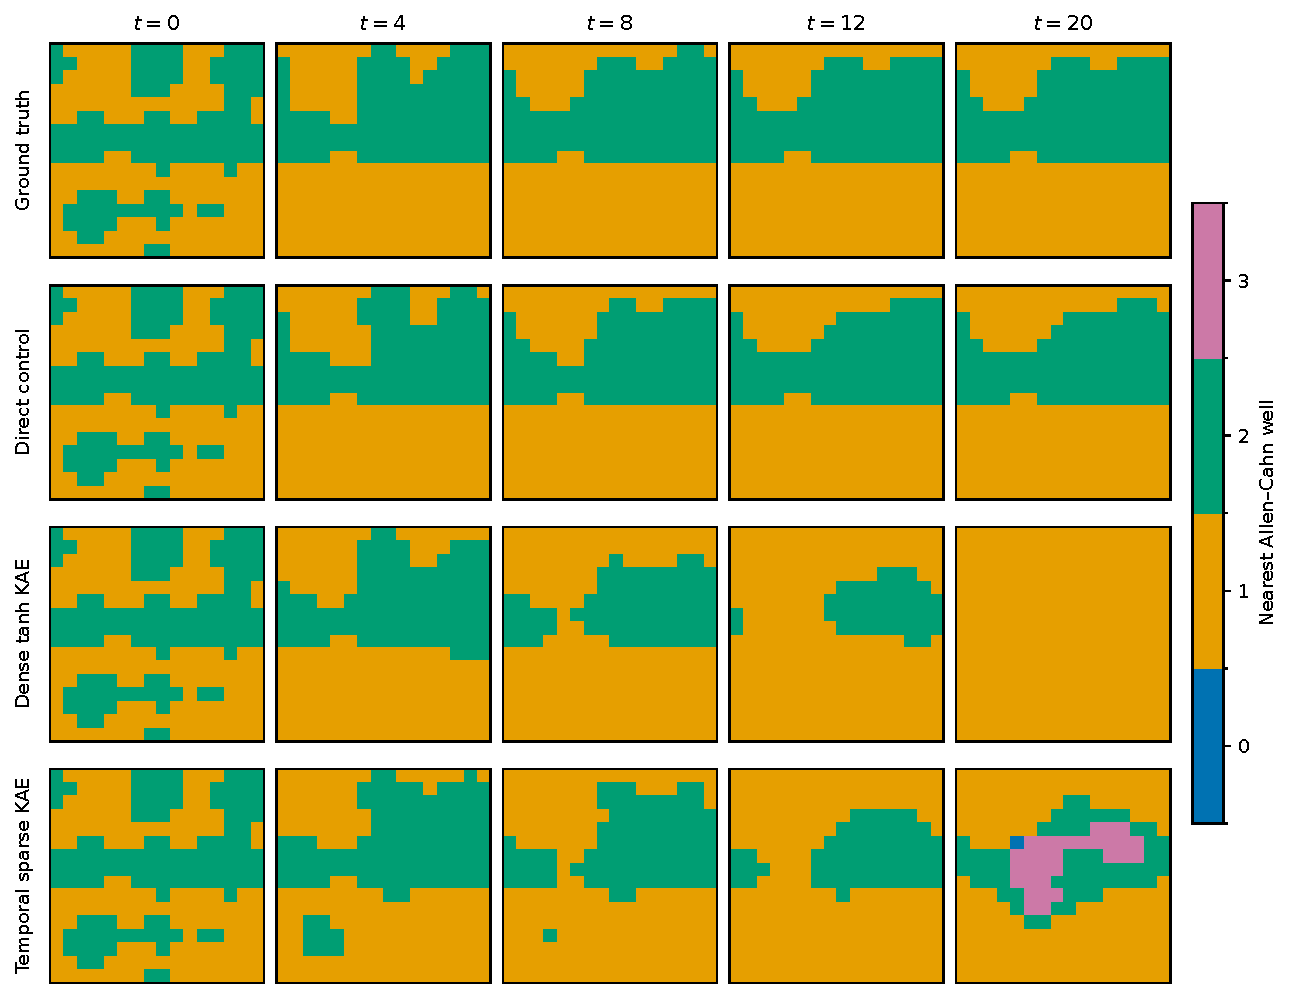
\includegraphics[width=\textwidth]{figures/neurips_paper_2026/fig_allen_cahn_time20_snapshots.pdf}
\caption{Predeclared qualitative long-horizon Allen--Cahn trajectory on the
new-simulation-seed holdout, shown as nearest-well maps at physical times through
$20$. The direct control preserves the evolving interface most faithfully;
the sign-split temporal-support KAE has the weakest long-horizon forecast. The trajectory
and model seed were fixed before the new holdout was opened and are not used
for quantitative selection.}
\label{fig:allen_cahn_time20_snapshots}
\end{figure*}

\paragraph{Inference.}
The Lorenz--96, Allen--Cahn temporal-support, forecast-optimized Allen--Cahn,
same-checkpoint new-IC, and secondary physical-metric packets average trajectories within model seed and use ten paired
model-initialization seeds as inferential units. Lorenz--96 and temporal-support
intervals use 100,000 percentile bootstrap resamples; their paired tests
enumerate all sign flips, with long-horizon $p$-values Holm-adjusted within each
declared family. The forecast-optimized packet instead uses 50,000 paired-seed
resamples of each ratio-of-arm-means reduction. Its four intervals are marginal
and its frozen primary decision is an intersection-union gate; the exact
one-sided 1,024-swap max-$t$ calculation is a multiplicity sensitivity over the
dependent H160/H200 mean/terminal cells (H160 is a prefix of H200), not a
replacement decision. Lorenz--96 and the original Allen--Cahn intervals
condition on one fixed evaluation dataset. The new-IC interval averages three
fixed datasets within each paired checkpoint seed. They quantify variation
across the ten trained seed pairs, but not an independent repeat of the
training/selection pipeline, a future retraining packet, PDE parameters,
resolutions, or physical systems. The new-IC
check crosses the three datasets with every checkpoint, averages them within
paired model seed, uses 100,000
paired-seed resamples, and enumerates the same 1,024 paired sign flips. Neither benchmark uses fate labels, basin counts, or
trajectory assignments for training, encoding, representative fitting, or
family transfer. In the temporal-support packet, validation fate metrics select
the T20 scope, Jaccard-0.40 rule, temporal weight, and advancement of the whole
fixed ten-seed packet; labels on the
new-simulation-seed holdout only score the frozen assignments and the
declared single-well-dominated final-field slice.
The physical-metric packet uses the same within-seed dataset averaging and
100,000 paired-seed resamples, one-sided exact sign flips, and Holm correction
over all seven H200 cumulative endpoints. Its two nonsignificant metrics and
all terminal and late-window summaries remain visible rather than being
removed from the family.

\clearpage
